\apendice{Documentación técnica de programación}

\section{Introducción}\label{introducción-manial-programador}

En este anexo se detalla la documentación técnica de programación, incluyendo la instalación del entorno de desarrollo, la estructura de la aplicación, su compilación, la configuración de los diversos servicios de integración utilizados y las baterías de pruebas realizadas.

\section{Estructura de directorios}\label{estructura-de-directorios}

El repositorio del proyecto tiene la siguiente estructura:

\begin{itemize}
    \item \textbf{/:} directorio raíz del repositorio. Es este se encuentra todos los directorios del proyecto además de una README.
    \item \textbf{/app:} directorio de la aplicación. Este contiene tanto la propia aplicación como aquellos directorios necesarios para la correcta ejecución de la misma.
    \item \textbf{/app/src:} directorio del código fuente de la aplicación.
    \item \textbf{/app/src/functions:} directorio de los scripts utilizados por el sistema.
    \item \textbf{/app/src/livescripts:} directorio de los livescripts y sus correspondientes HTML de la documentación de dentro de la aplicación tanto en español como en inglés.
    \item \textbf{/app/src/livescripts/img:} directorio de las imágenes utilizadas en la documentación de los livescripts.
    \item \textbf{/app/src/test:} directorio de los tests unitarios de los scripts de `/functions'. Cuentan con un README para poderlos ejecutar correctamente.
    \item \textbf{/app/data:} directorio de las imágenes proporcionadas y sus respectivas imágenes ground truth, además contiene un README para explicar la nomenclatura utilizada en las imágenes.
    \item \textbf{/app/data/Imagenes:} directorio de las imágenes proporcionadas por la aplicación.
    \item \textbf{/app/data/Imagenes\_ground\_truth:} directorio de las imágenes ground truth correspondientes a las imágenes proporcionadas por la aplicación.
    \item \textbf{/app/cache:} directorio de la memoria caché de la aplicación. En el se guardaran las imágenes generadas durante la ejecución.
    \item \textbf{/app/results:} directorio donde se almacenaran las imágenes por defecto si el usuario decide guardar los resultados de la ejecución.
    \item \textbf{/docs:} directorio de la documentación del proyecto.
    \item \textbf{/docs/img:} directorio de las imágenes utilizadas en la documentación.
    \item \textbf{/docs/tex:} directorio de las fuentes en formato \LaTeX para memoria y anexos.
\end{itemize}

\section{Manual del programador}\label{manual-del-programador}

El siguiente manual tiene como objetivo explicar cómo un programador puede descargar el proyecto y desarrollar su propia versión.

\subsection{Entorno de desarrollo}\label{entorno-de-desarrollo}

Para poder trabajar con el proyecto es necesario tener instalado esta serie de programas y dependencias.

\begin{itemize}
    \item MATLAB 2023b.
    \item MATLAB Add-On Toolboxes.
    \item GitHub Desktop.
\end{itemize}

A continuación, se detallan las instrucciones para instalar y configurar correctamente cada uno de ellos.

\subsubsection{MATLAB 2023b}\label{matlab-2023b}

El principal e indispensable programa para la ejecución de este proyecto es MATLAB, más concretamente la versión 2023b. Para descargarlo tenemos que ir a la página oficial de MATLAB \cite{matlab2023b}. Una vez iniciada la aplicación, se pedirá introducir una cuenta de MATLAB. La Universidad de Burgos ofrece a los alumnos acceso a la versión académica de MATLAB con su correo institucional, versión con la cual se ha realizado este proyecto.

\subsubsection{MATLAB Add-On Toolboxes}\label{matlab-toolboxes}

Una vez instalado MATLAB, será necesario instalar una serie de Add-On Toolboxes para la correcta ejecución del proyecto. Estas son las siguientes:

\begin{itemize}
    \item Statistics and Machine Learning Toolbox.
    \item Fuzzy Logic Toolbox.
    \item HMRF-EM-image.
    \item MATLAB Compiler.
\end{itemize}

Esto se puede hacer desde el menú superior APPS' y luego pulsando en Get More Apps'. A continuación, se mostrará una nueva ventana donde, mediante un buscador, se podrá acceder a las Add-On Toolboxes necesarias. A continuación, se muestra un ejemplo de la instalación de `Statistics and Machine Learning Toolbox' en la figura \ref{fig:descarga_toolboxes}.

\imagen{descarga_toolboxes}{Instalación Statistics and Machine Learning Toolbox}

En la figura \ref{fig:descarga_toolboxes} se muestra la ventana que se obtiene tras instalar Statistics and Machine Learning Toolbox.

\subsubsection{GitHub Desktop}\label{github-desktop}

La instalación de GitHub Desktop no es estrictamente necesaria pero sí recomendable ya que permite tener un control de versiones lo cual es de gran interés a la hora de hacer cambios en la aplicación.

Para instalar GitHub Desktop, se debe ir a la página oficial \cite{githubDesktop} y desde allí descargar los archivos necesarios. Tras la instalación, se pedirá ingresar el usuario de GitHub

\subsection{Descarga del repositorio}\label{descarga-del-repositorio}

Para la descarga del repositorio hay dos principales opciones:

\subsubsection{Obtención manual del código fuente}\label{obtención-manual-del-código-fuente}

En el caso de que no estimemos necesario un control de versiones, se puede descargar directamente el archivo .zip del proyecto desde el repositorio de GitHub (\url{https://github.com/jms1008/TFG-Invariantes-de-iluminacion-en-piezas-metalicas}). Esto se realiza pulsando en el botón `Code' y más tarde en el de `Download ZIP' como se puede ver en la figura \ref{fig:descarga_zip}:

\imagen{descarga_zip}{Descarga del repositorio mediante el entorno web.}

En la figura \ref{fig:descarga_zip} se muestra donde está ubicado el botón para poderse descargar el repositorio desde GitHub.

Tras esto solo quedaría descomprimir el proyecto en el directorio deseado.

\subsubsection{Obtención del código fuente mediante GitHub Desktop}\label{pbtención-del-código-fuente-mediante-github-desktop}

El el caso de querer tener un control de versiones, se puede utilizar la aplicación GitHub Desktop mencionada anteriormente en \ref{github-desktop}.

Para ello, se debe entrar a la aplicación, pulsar en `Clonar repositorio' e introducir el enlace del proyecto que se desea clonar. En este caso, el enlace del repositorio de este proyecto es el siguiente: \url{https://github.com/jms1008/TFG-Invariantes-de-iluminacion-en-piezas-metalicas}. A continuación, se debe indicar dónde se desea almacenar el repositorio.

\subsection{Importación del proyecto}\label{importación-del-proyecto}

Para la correcta ejecución del proyecto, se debe abrir MATLAB 2023b y navegar dentro de MATLAB al directorio donde se encuentre el repositorio. Una vez allí, se debe escribir en la consola `appdesigner' para que se abra la ventana correspondiente, donde se podrá visualizar, modificar y ejecutar, entre muchas otras funcionalidades, la aplicación.

\subsubsection{MATLAB App Designer}\label{matlab-app-designer}

La en la primera pantalla que aparece nada más abrir MATLAB App Designer nos permitirá abrir un proyecto. Aquí hemos de seleccionar el archivo `InvIPM.mlapp' que se encuentra en el directorio `/app'.

Una vez abierto el proyecto veremos una vista de diseño de la aplicación donde se puede modificar la posición y algunos valores dentro del apartado visual como se muestra en la figura \ref{fig:MATLAB_App_Designer} y otro botón que permite acceder a la vista de código.

\imagen{MATLAB_App_Designer}{Ventana principal de MATLAB App Designer.}

La figura \ref{fig:MATLAB_App_Designer} muestra la interfaz que muestra MATLAB tras abrir el proyecto descargado previamente.

Es en la vista de código donde se podrá modificar más en profundidad los objetos visuales y programar las funcionalidades de las distintas interacciones de la aplicación.

Aunque la forma de programar en MATLAB App Designer es muy similar a la programación en MATLAB, hay una serie de cambios y funcionalidades que son muy relevantes. En el siguiente enlace se encuentra una guía de las funcionalidades y la forma de programar en MATLAB App Designer, \url{https://es.mathworks.com/help/matlab/app-designer.html}

\section{Compilación, instalación y ejecución del proyecto}\label{compilación-instalación-ejecución}

A continuación, se explicará cómo:

\begin{itemize}
    \item Compilar y ejecutar el proyecto dentro de MATLAB.
    \item Crear una nueva release mediante una MATLAB Standalone Application.
    \item Directorios creados por el compilador de MATLAB.
    \item Ejecución de la Standalone App.
\end{itemize}

\subsection{Compilación en App Designer}\label{compilación-en-app-designer}

MATLAB permite ejecutar directamente desde la interfaz compilar y ejecutar la aplicación. Para ello simplemente tendremos que pulsar el icono de `run' que se encuentra en la barra superior, dicho icono es el que se muestra en la figura \ref{fig:play_in_MATLAB}.

\imagen{play_in_MATLAB}{Icono de compilación y ejecución de MATLAB App Designer.}

La figura \ref{fig:play_in_MATLAB} muestra la ubicación en la interfaz del botón que se utiliza para compilar y ejecutar la app.

Tras esto, se abrirá la aplicación en una ventana emergente donde se podrán probar de forma muy sencilla las distintas funcionalidades que sean añadidas. Dicha ventana tendrá un aspecto similar al mostrado en la figura \ref{fig:aplicacion_compilada}

\imagen{aplicacion_compilada}{Ventana de la aplicación compilada y ejecutada.}

La figura \ref{fig:aplicacion_compilada} muestra ventana que se crea automáticamente tras la compilación y ejecución de la aplicación.

\subsection{Crear una nueva release}\label{crear-una-nueva-release}

Tras realizar las pertinentes modificaciones o añadir nuevas funcionalidades a la aplicación, el siguiente paso será compartir la aplicación. MATLAB para ello tiene tres opciones:

\begin{itemize}
    \item \textbf{MATLAB App:} esta opción permite crear una archivo de instalación para compartir la aplicación con otros usuarios de MATLAB. Si el objetivo es que estos puedan modificar o ver el funcionamiento del código, esta es la mejor opción.
    \item \textbf{Web App:} esta opción permite crear y desplegar aplicaciones web utilizando MATLAB Compiler, facilitando su distribución y uso en diferentes entornos. Esto ha sido desestimado ya que esta funcionalidad la ofrece pero es de pago.
    \item \textbf{Standalone Desktop App:} esta opción permite crear aplicaciones de escritorio independientes usando MATLAB Compiler, que requieren tener MATLAB instalado para su ejecución. Esta es la opción que se ha utilizado y que se desarrollará con más detalle a continuación.
\end{itemize}

\subsubsection{MATLAB Standalone Application}\label{matlab-standalone-application}

Para crear una Standalone Application dentro de MATLAB App Designer, se debe pulsar el icono de compartir y, a continuación, seleccionar la opción de `Standalone Desktop App'. Tras esto, aparecerá una ventana para añadir la información relevante de la aplicación que se va a crear. Aquí se deben introducir los siguientes datos, como se muestra en la figura \ref{fig:standalone_app}:

\begin{itemize}
    \item Nombre de la aplicación.
    \item Versión de la aplicación.
    \item Autor (nombre, correo, compañía).
    \item Descripción (opcional).
    \item Archivos y directorios necesarios para la correcta ejecución del programa.
    \item Archivos visibles para el usuario.
\end{itemize}

\begin{figure}[h!]
  \centering
  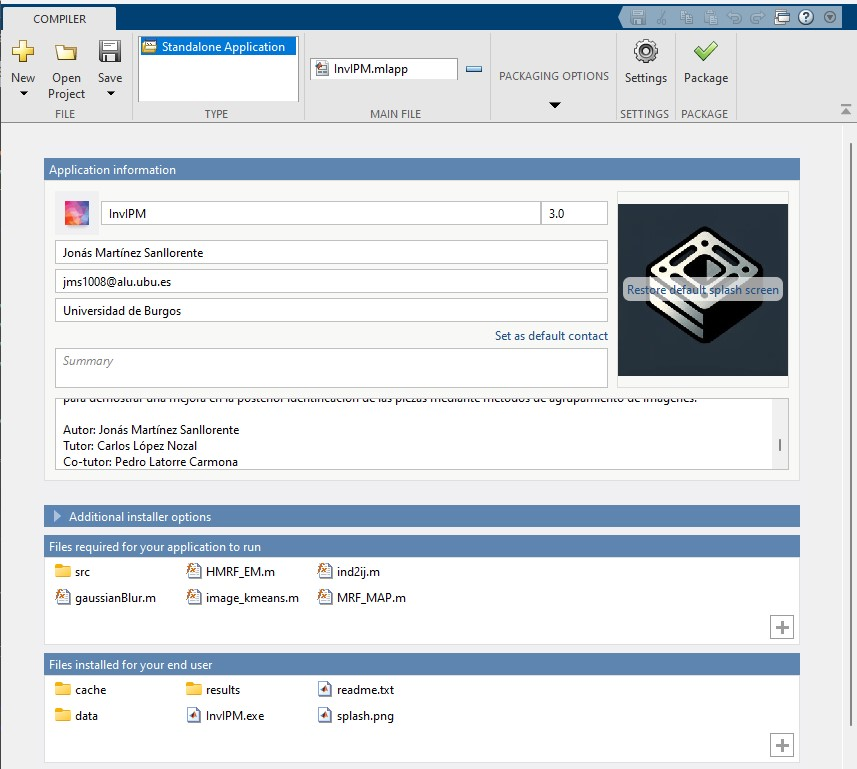
\includegraphics[scale=0.4]{standalone_app}
  \caption{Creación de MATLAB Standalone App.}
  \label{fig:standalone_app}
\end{figure}

La figura \ref{fig:standalone_app} muestra la interfaz que MATLAB ofrece para la creación de una Standalone App.

\subsubsection{Ejecución de la Standalone App}\label{ejecución-de-la-standalone-app}

Al abrir el archivo `InvIPM.exe', se accederá a la aplicación, la cual ejecutará todos los scripts y el código de manera transparente para el usuario, mostrando únicamente los directorios deseados. En este caso, estos serían:

\begin{itemize}
    \item El directorio `/data' ya que contienen las imágenes de prueba con sus respectivas imágenes ground truth.
    \item El directorio `/cache' ya que sera donde se almacenen todos los resultados de antiguas ejecuciones de forma temporal.
    \item El directorio `/results' ya que sera la ruta por defecto que se le ofrezca al usuario cuando este desee guardar los resultados de una ejecución.
    \item El README con las pertinentes explicaciones.
    \item El splash de la aplicación.
\end{itemize}

\section{Pruebas del sistema}\label{pruebas-del-sistema}

A continuación, se desarrollarán las distintas pruebas del sistema.

\subsection{Casos de prueba}\label{casos-de-prueba}

Se han creado múltiples tests unitarios para comprobar el correcto funcionamiento de manera aislada de los scripts que utiliza la aplicación.

Los distintos tests creados son los siguientes:

\begin{itemize}
    \item alvarez\_transformTest.m
    \begin{itemize}
        \item Test básico.
        \item Test de valores extremos.
        \item Test con una imagen uniforme.
        \item Test con una imagen en blanco y negro.
    \end{itemize}
    \item maddern\_transformTest.m
    \begin{itemize}
        \item Test básico.
        \item Test de valores extremos.
        \item Test con una imagen uniforme.
    \end{itemize}
    \item krajnik\_transformTest.m
    \begin{itemize}
        \item Test básico.
        \item Test de valores extremos.
        \item Test con una imagen uniforme.
    \end{itemize}
    \item upcroft\_transformTest.m
    \begin{itemize}
        \item Test básico.
        \item Test de valores extremos.
        \item Test con una imagen uniforme.
    \end{itemize}
    \item calcular\_alphaTest.m
    \begin{itemize}
        \item Test valores básicos.
        \item Test con lambda1 a 0.
        \item Test con las tres lambdas iguales.
    \end{itemize}
    \item calcular\_theta\_krajnikTest.m
    \begin{itemize}
        \item Test valores básicos.
        \item Test con una imagen uniforme.
        \item Test con una imagen en blanco y negro.
    \end{itemize}
    \item calcular\_coincidenciaTest.m
    \begin{itemize}
        \item Test con imágenes iguales.
        \item Test con imágenes diferentes.
    \end{itemize}
    \item check\_cacheTest.m
    \begin{itemize}
        \item Test existe caché (la crea, añade una imagen y luego borra la caché).
    \end{itemize}
    \item convertir\_a\_blanco\_negro\_con\_bordesTest.m
    \begin{itemize}
        \item Test con un caso perfecto.
        \item Test con un caso no perfecto.
    \end{itemize}
    \item imagen\_tres\_canalesTest.m
    \begin{itemize}
        \item Test con una imagen de cuatro canales.
        \item Test con una imagen de tres canales.
    \end{itemize}
    \item metodos\_agrupamientoTest.m
    \begin{itemize}
        \item Test de K-Means sin imagen ground truth.
        \item Test de K-Means con imagen ground truth.
    \end{itemize}
    \item metodos\_invariantesTest.m
    \begin{itemize}
        \item Test de el invariante de Álvarez.
        \item Test de el invariante de Maddern.
    \end{itemize}
    \item moda\_colorTest.m
    \begin{itemize}
        \item Test básico, un color aparece repetido.
        \item Test de colores únicos.
    \end{itemize}
    \item segmentar\_imagen\_fuzzy\_CMeansTest.m
    \begin{itemize}
        \item Test básico.
    \end{itemize}
    \item segmentar\_imagen\_GMMTest.m
    \begin{itemize}
        \item Test básico.
    \end{itemize}
    \item segmentar\_imagen\_KMeansTest.m
    \begin{itemize}
        \item Test básico.
    \end{itemize}
\end{itemize}

Como se puede apreciar, ni PCA ni HMRF\_EM tienen test unitarios propios ya que dichas librerías ya han sido testeadas por sus desarrolladores.

\subsection{Ejecución de los casos de prueba}\label{ejecución-de-los-casos-de-prueba}

Para ejecutar los casos de prueba, como viene indicado en el README de la carpeta test, hay de copiar los scripts del directorio `/test' al directorio `/functions'.

Una ver realizado esto tenemos dos opciones.
\begin{enumerate}
    \item \textbf{Ejecutar uno a uno:} si se desea ejecutar un test específico por separado, se debe abrir la consola de comandos y utilizar el siguiente comando, reemplazando `nombreDelTest' por el nombre del test que deseas ejecutar `disp(runtests(`nombreDelTest'))'.
    \item \textbf{Ejecutar todos a la vez:} si se desea ejecutar todos los tests a la vez, simplemente se debe ejecutar el archivo `run\_all\_tests.m'. Este archivo se encargará de correr todos los tests de forma automática.
    
    Los resultados de ejecutar todos los tests son los que se pueden observar en la figura \ref{fig:resultados_tests}.
\end{enumerate}

\imagen{resultados_tests}{Resultados de la ejecución de los tests.}

La figura \ref{fig:resultados_tests} muestra un resumen de los resultados de la ejecución de los tests sobre los scripts que utiliza la aplicación.